\documentclass[t]{beamer}
%\usetheme{iclpt}
\usepackage{url}
\usepackage{pifont}
\usepackage{amscd}
\usepackage{MnSymbol}
\newcommand{\tick}{{\color{green}\ding{51}}}
\newcommand{\dcross}{{\color{red}\ding{55}$\,$}}
\usepackage{pythonhighlight}
\newcommand{\dd}[2]{\frac{\diff#1}{\diff #2}} 
\def\MM#1{\boldsymbol{#1}}
\beamertemplatenavigationsymbolsempty
\author[Colin Cotter]{Prof. Colin Cotter}
\institute{Imperial College London}
\DeclareMathOperator{\diff}{d\!}
\DeclareMathOperator{\Div}{div}
\DeclareMathOperator{\Id}{Id}
\DeclareMathOperator{\Ro}{Ro}
\DeclareMathOperator{\ccurl}{curl}
\DeclareMathOperator{\ddiv}{div}
\DeclareMathOperator{\Tr}{Tr}
\newcommand{\pp}[2]{\frac{\partial #1}{\partial #2}} 
\newcommand{\Hcurl}{H(\operatorname{curl})}
\newcommand{\Hdiv}{H(\operatorname{div})}
\newcommand{\comment}[1]{}
\newcommand{\jump}[1]{\left[\!\left[ #1 \right]\!\right]}
\title[CCMI]{Project topic: PDE-driven Digital Twins\\
  \vspace{5mm}
  
\includegraphics[width=4cm]{ccmi_square_colour_text}
  \hspace{5mm}
  
\includegraphics[width=4cm]{ukri_logo}}

\newtheorem{proposition}[theorem]{Proposition}
\newcommand{\dede}[2]{\frac{\delta #1}{\delta #2}}
\newenvironment{packed_enum}{
\begin{enumerate}
  \setlength{\itemsep}{1pt}
  \setlength{\parskip}{0pt}
  \setlength{\parsep}{0pt}
}{\end{enumerate}}

\newcommand{\V}{\mathbf{V}}
\newcommand{\U}{\mathbf{U}}
\newcommand{\W}{\mathbf{W}}
\newcommand{\M}{\mathrm{M}}
\newcommand{\R}{\mathrm{R}}
\newcommand{\La}{\mathrm{L}}
\newcommand{\Fu}{\mathbf{F}}


\usepackage{tikz}
\usepackage{amsmath}
\usetikzlibrary{trees,positioning}

\newenvironment{packed_item}{
\begin{itemize}
  \setlength{\itemsep}{1pt}
  \setlength{\parskip}{0pt}
  \setlength{\parsep}{0pt}
}{\end{itemize}}

\begin{document}

\date{}

\frame{\maketitle}

\frame{
  \frametitle{Digital Twins}
  \begin{center}
    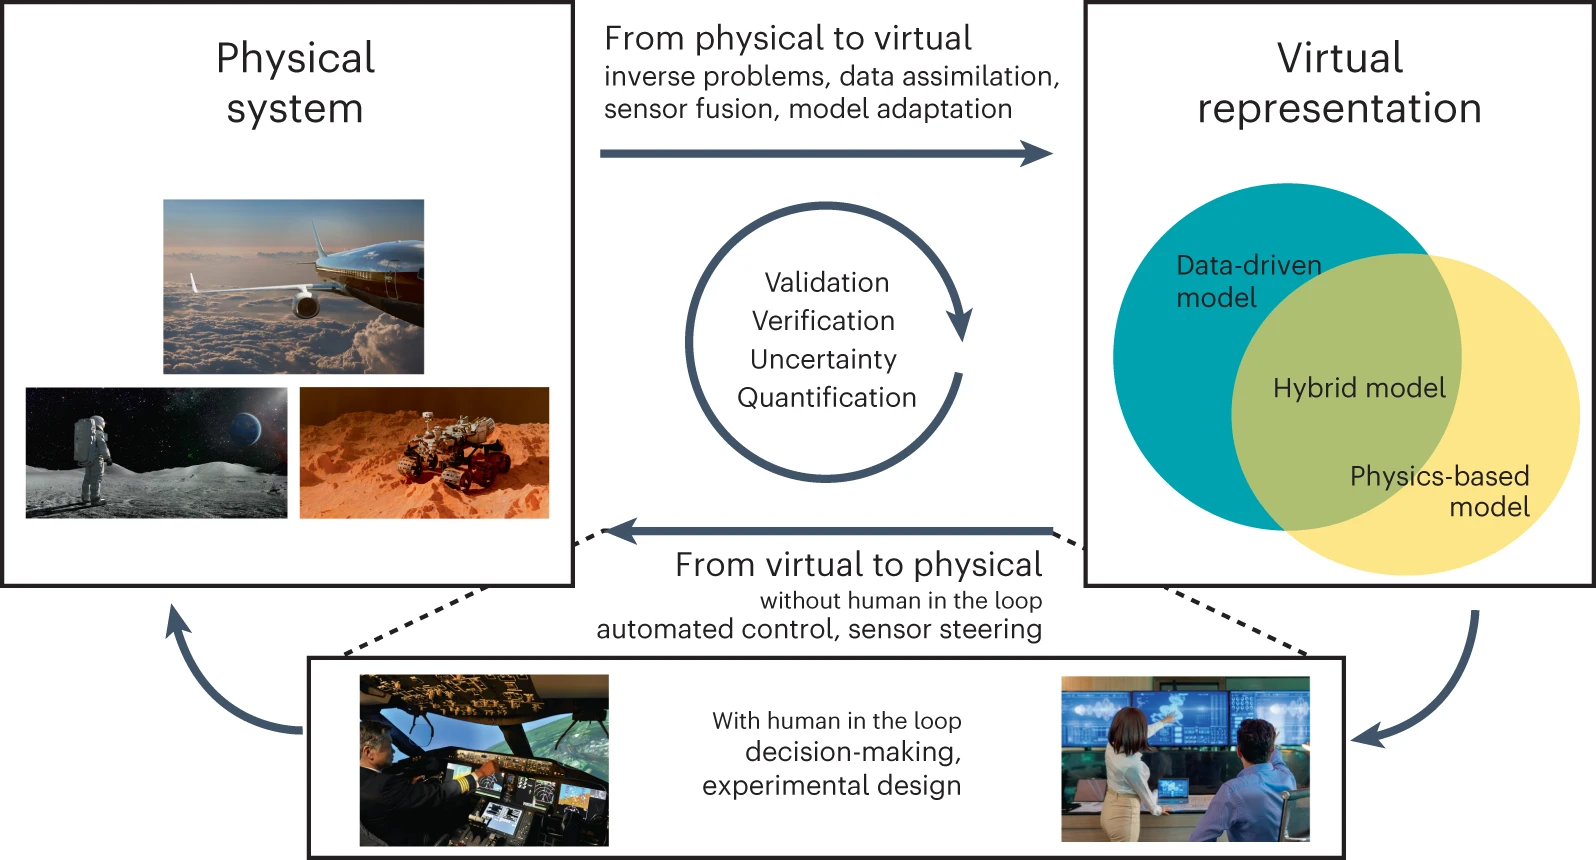
\includegraphics[width=8cm]{43588_2024_613_Fig1_HTML}\\
    \footnotesize{Ferrari and Willcox (2024)}
  \end{center}
  \begin{block}{AIAA Digital Engineering Integration Committee (2020)}
    “a set of virtual information constructs that mimics the
    structure, context, and behavior of an individual or unique
    physical asset, is dynamically updated with data from its physical
    twin throughout its life cycle, and ultimately informs decisions
    that realize value”.
  \end{block}
}

\frame{
  \frametitle{Trade-offs}
  \vfill
  \centerline{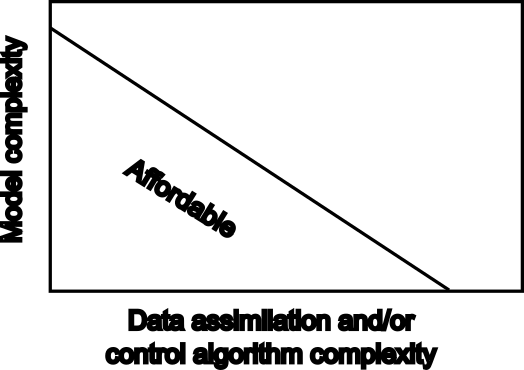
\includegraphics[width=6cm]{complexity}}
  \begin{block}{}
     In this project we will explore mathematical aspects of this
    tradeoff in the functional setting: the idealised system state is
    represented by one or more functions of space and can be modelled
    by a partial differential equation (or another functional process)
  \end{block}
  \vfill
}

\frame{
  \frametitle{Some possible tools for model reduction/surrogates}
  \begin{itemize}
  \item Multilevel algorithms,
  \item generative models,
  \item neural operators,
  \item stochastic parameterisation,
  \item \emph{etc.}
  \end{itemize}
}

\frame{
  \frametitle{Some possible idealised application systems}
  \begin{itemize}
  \item Experimental wave tank facility
  \item Flood catchment
  \item Coastal zone
  \item Chemical pipeflow
  \item Something else!
  \end{itemize}
}

\frame{
  \vfill
  \centerline{The End}
  \vfill
}

\end{document}
